\section{Lecture 17 \& 18: Linear Transformation, Kernel \& Range}
\rmk{
    This lecture covers: 
    \begin{itemize}
        \item 6.1 Definition of Linear Transformations
        \item 6.2 Transformations of $\mathbb{R}^2$
        \item 6.3 The Kernel and Range of a Linear Transformation
    \end{itemize}
}

\subsection{Definition of Linear Transformations}
\subsubsection{Definition}
\defn{Mapping}{
    Let $V$ and $W$ be vector spaces. A \textbf{mapping} $T$ from $V$ to $W$ is a rule that assigns to each vector $\vec{v}$ in $V$ precisely one vector $\vec{w} = T(\vec{v})$. We write $T: V \to W$.
}

Linear Transformation is a kind of mapping that preserves the operations of vector addition and scalar multiplication.

\defn{Linear Transformation}{
    Let $V$ and $W$ be vector spaces over the same field. A mapping $T: V \to W$ is a \textbf{linear transformation} if for all $\vec{v}_1, \vec{v}_2 \in V$ and all scalars $c$:
    \begin{enumerate}
        \item $T(\vec{u} + \vec{v}) = T(\vec{u}) + T(\vec{v})$ for all $\vec{u}, \vec{v} \in V$
        \item $T(c\vec{v}) = cT(\vec{v})$ for all $\vec{v} \in V$
    \end{enumerate}
    In the above equations, the operations on the left of the equal signs are the ones defined in the domain $V$ and
the ones on the right of the equal signs are the ones defined in the codomain $W$.
}

\begin{figure}
    \center
    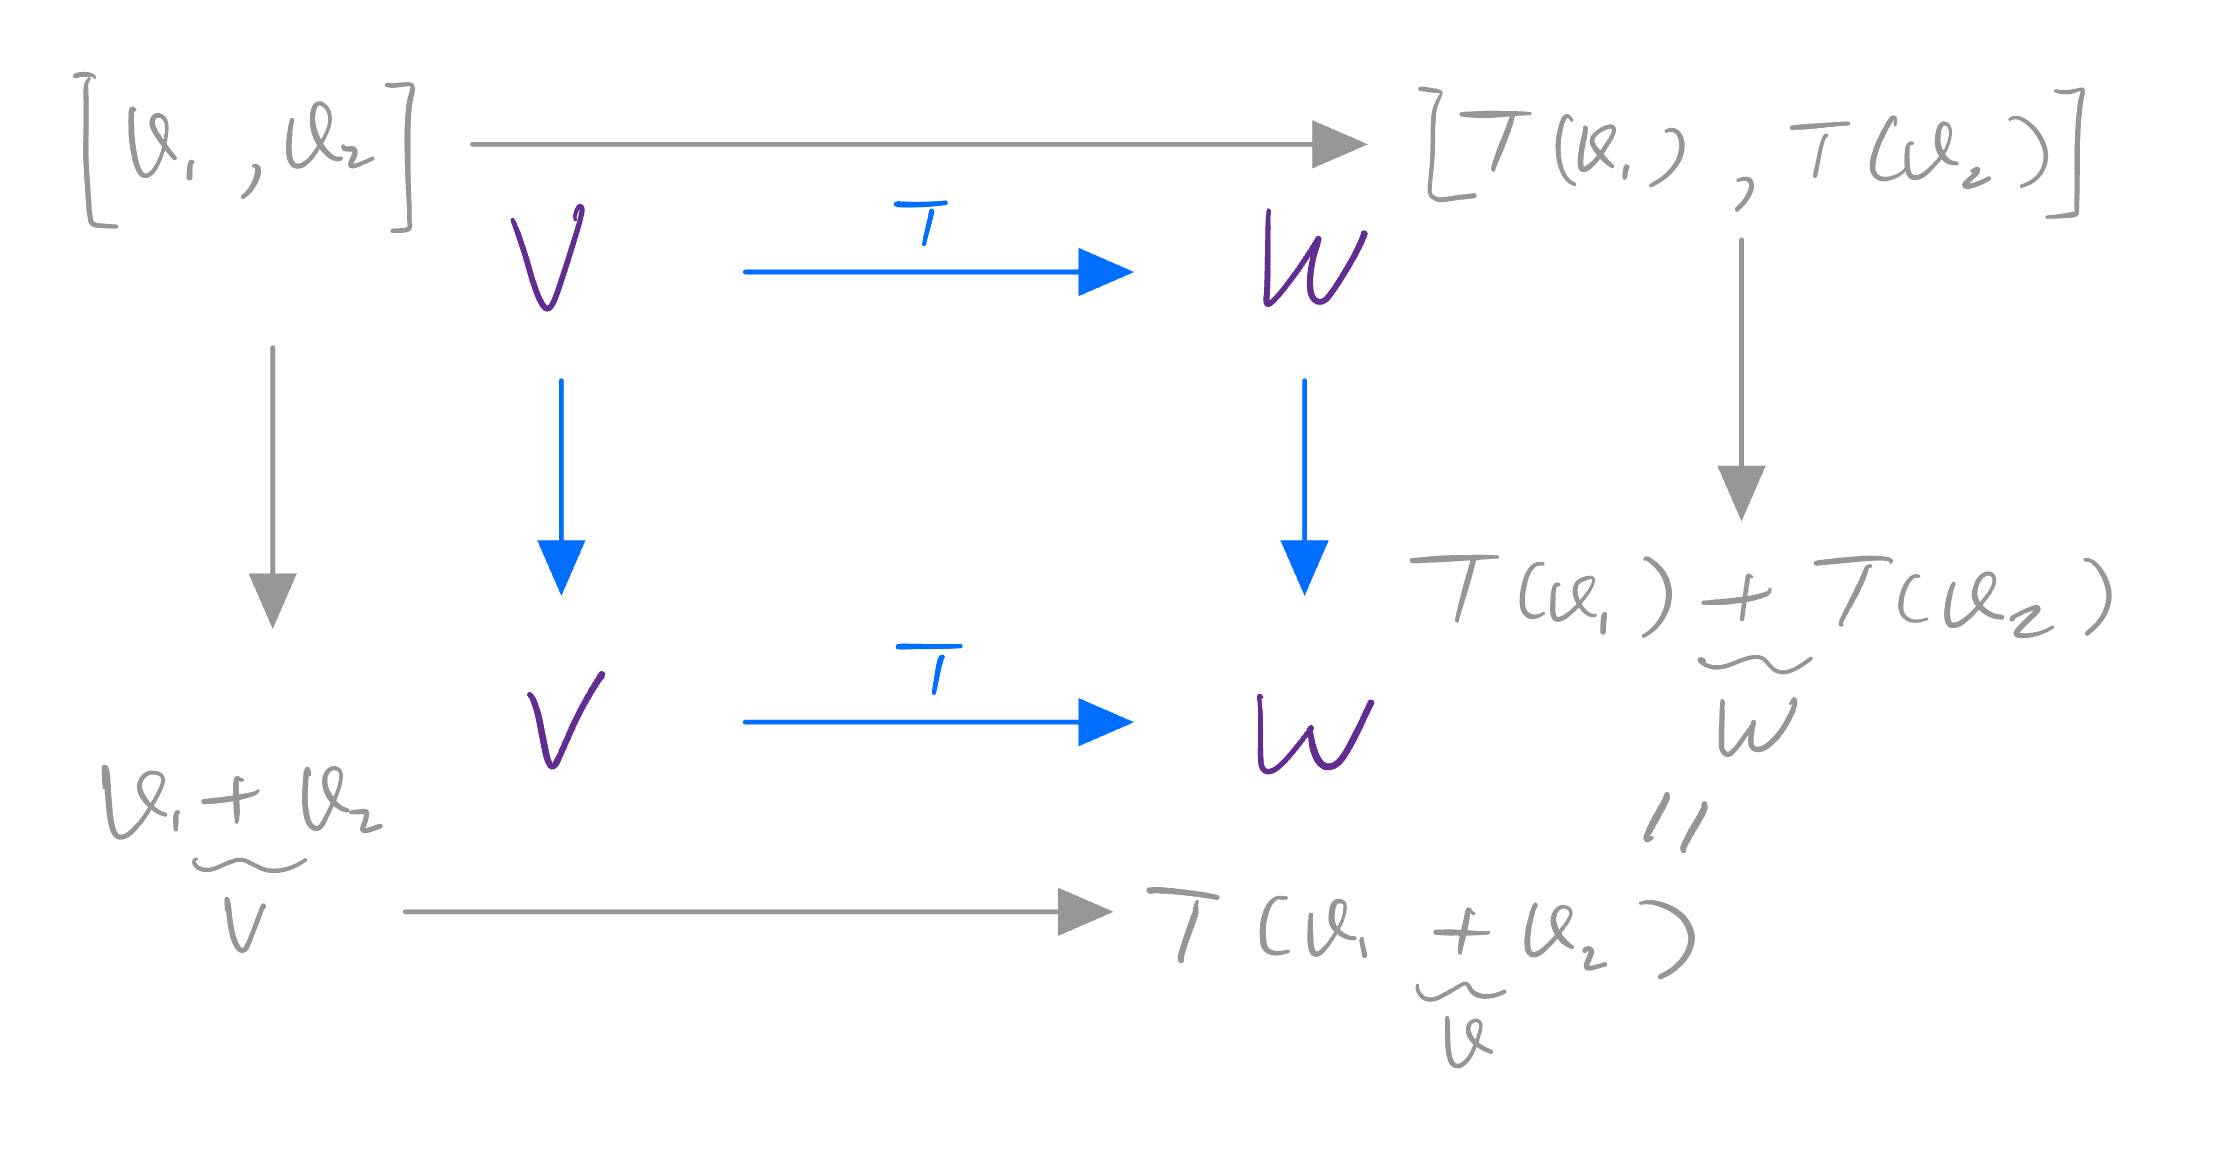
\includegraphics[width=0.5\textwidth]{img/Note 25 Mar 2024.jpeg}
    \caption{Linear Transformation Diagram}
\end{figure}
\subsection{How to prove a transformation is linear}

\ex{
    Show $T:P_2 \to P_4$ given by $T(p) = x^2 p(x)$ is linear. 
    \begin{proof}
        We need to show that $T(p + q) = T(p) + T(q)$ and $T(cp) = cT(p)$ for all $p, q \in P_2$ and $c \in \mathbb{R}$. \\
        Let $p, q \in P_2$ and $c \in \mathbb{R}$. \\
        \[
            T(p + q) = x^2(p + q)(x) = x^2p(x) + x^2q(x) = T(p) + T(q)
        \]
        \[T(cp) = x^2(cp)(x) = cx^2p(x) = cT(p)\]
        Thus, $T$ is linear.

    \end{proof}

}

Here's a short-cut to test if a transformation is linear:

\thmr{}{}{
    Let $V, W$ be vector spaces over field $F$. A mapping $T: V \to W$ is a linear transformation if and only if for all $\lambda_1, \lambda_2 \in F$ and all $\vec{v}_1, \vec{v}_2 \in V$:
    \[
        T(\lambda_1\vec{v}_1 + \lambda_2\vec{v}_2) = \lambda_1T(\vec{v}_1) + \lambda_2T(\vec{v}_2)
    \]
}



\ex{
    Which of the following are linear transformations?
\begin{enumerate}
    \item $T: P_2 \to P_1$ given by $T(p) = p'$
    \item $T: \mathbb{R} \to \mathbb{R}^2$ given by $T(x) = (x, 2x)$
    \item $T: \mathbb{R} \to \mathbb{R}^2$ given by $T(x) = (x, x^2)$
\end{enumerate}
\begin{proof} We can use the definition of linear transformations to check each case: 
    \begin{enumerate}
        \item $T(p) = p'$ is linear since $T(\lambda_1p_1 + \lambda_2p_2) = (\lambda_1p_1 + \lambda_2p_2)' = \lambda_1p_1' + \lambda_2p_2' = \lambda_1T(p_1) + \lambda_2T(p_2)$
        \item $T(x) = (x, 2x)$ is linear since $T(\lambda_1x_1 + \lambda_2x_2) = (\lambda_1x_1 + \lambda_2x_2, 2(\lambda_1x_1 + \lambda_2x_2)) = \lambda_1(x_1, 2x_1) + \lambda_2(x_2, 2x_2) = \lambda_1T(x_1) + \lambda_2T(x_2)$
        \item $T(x) = (x, x^2)$ is not linear since $T(\lambda_1x_1 + \lambda_2x_2) = (\lambda_1x_1 + \lambda_2x_2, (\lambda_1x_1 + \lambda_2x_2)^2) \neq \lambda_1(x_1, x_1^2) + \lambda_2(x_2, x_2^2) = \lambda_1T(x_1) + \lambda_2T(x_2)$
    \end{enumerate}
\end{proof}
}


\ex{
    $T: \mathbb{R}^2 \to P_1(\mathbb{R})$ given by $T(a, b) = a + bx$ is linear.
    \begin{proof}
        We want to show: $T(\lambda_1(a_1, b_1) + \lambda_2(a_2, b_2)) = \lambda_1T(a_1, b_1) + \lambda_2T(a_2, b_2)$
        \[
            T(\lambda_1(a_1, b_1) + \lambda_2(a_2, b_2)) = T(\lambda_1a_1 + \lambda_2a_2, \lambda_1b_1 + \lambda_2b_2) = (\lambda_1a_1 + \lambda_2a_2) + (\lambda_1b_1 + \lambda_2b_2)x
        \]
        \[
            \lambda_1T(a_1, b_1) + \lambda_2T(a_2, b_2) = \lambda_1(a_1 + b_1x) + \lambda_2(a_2 + b_2x) = (\lambda_1a_1 + \lambda_2a_2) + (\lambda_1b_1 + \lambda_2b_2)x
        \] \\
        Therefore, $T(\lambda_1(a_1, b_1) + \lambda_2(a_2, b_2)) = \lambda_1T(a_1, b_1) + \lambda_2T(a_2, b_2)$ \\
        Thus, $T$ is linear.
    
    \end{proof}
        
}

\subsubsection{Three very important examples of linear transformations}
\ex{
    \textbf{1:} A transformation given by a matrix: $T : \mathbb{R}^n \to \mathbb{R}^m$ given by $T(x) = Ax$ where $A$ is a fixed $m \times n$ matrix. \\
    \rmkb{Note that the domain of $T$ is $\mathbb{R}^n$ and the codomain is $\mathbb{R}^m$ – we reverse the order in which the dimensions of $A$ are listed.} \\
    Check that $T$ is linear:
    \pf{
        We want to show: $T(\lambda_1v_1 + \lambda_2v_2) = \lambda_1T(v_1) + \lambda_2T(v_2)$ \\
        Let $v_1, v_2 \in \mathbb{R}^n$ and $\lambda_1, \lambda_2 \in \mathbb{R}$. \\
        \[
            T(\lambda_1v_1 + \lambda_2v_2) = A(\lambda_1v_1 + \lambda_2v_2) = \lambda_1Av_1 + \lambda_2Av_2 = \lambda_1T(v_1) + \lambda_2T(v_2)
        \]
        Therefore, $T$ is linear. 
    } 
}

\ex{
    \textbf{2:} Differentiation: $D : C^1(\mathbb{R}) \to C(\mathbb{R})$ given by $D(f) = f'$. \\
    Check that $D$ is linear:
    \pf{
        We want to show: $D(\lambda_1f_1 + \lambda_2f_2) = \lambda_1D(f_1) + \lambda_2D(f_2)$ \\
        Let $f_1, f_2 \in C^1(\mathbb{R})$ and $\lambda_1, \lambda_2 \in \mathbb{R}$. \\
        \[
            D(\lambda_1f_1 + \lambda_2f_2) = (\lambda_1f_1 + \lambda_2f_2)' = \lambda_1f_1' + \lambda_2f_2' = \lambda_1D(f_1) + \lambda_2D(f_2)
        \]
        Therefore, $D$ is linear. 
    }
} 

\ex{
    \textbf{3:} The Identity map: $I : V \to V$ is defined by $I(v) = v$. For example when $V = \mathbb{R}$ the identity map is $I(x) = x$. \\
    Check that $I$ is linear:
    \pf{
        We want to show: $I(\lambda_1v_1 + \lambda_2v_2) = \lambda_1I(v_1) + \lambda_2I(v_2)$ \\
        Let $v_1, v_2 \in V$ and $\lambda_1, \lambda_2 \in \mathbb{R}$. \\
        \[
            I(\lambda_1v_1 + \lambda_2v_2) = \lambda_1v_1 + \lambda_2v_2 = \lambda_1I(v_1) + \lambda_2I(v_2)
        \]
        Therefore, $I$ is linear. 
    }
}

More example of proofing a transformation is linear:
\ex{
    Show $T: P_2 \to P_4 $ given by $T(p) = x^2p(x)$ is linear.
    \begin{proof}
        We want to show that $T(\lambda_1p_1 + \lambda_2p_2) = \lambda_1T(p_1) + \lambda_2T(p_2)$ \\
        Let $p_1, p_2 \in P_2$ and $\lambda_1, \lambda_2 \in \mathbb{R}$. \\
        \[
            T(\lambda_1p_1 + \lambda_2p_2) = x^2(\lambda_1p_1 + \lambda_2p_2)(x) = \lambda_1x^2p_1(x) + \lambda_2x^2p_2(x) = \lambda_1T(p_1) + \lambda_2T(p_2)
        \]

        Therefore, $T$ is linear.
    \end{proof} 
}

An example of a transformation that is not linear:

\rmkb{
    Notice that when disproving a transformation is linear, we only need to find one counterexample. (i.e. one pair of vectors and one scalar that does not satisfy the properties of linearity)
}

\ex{
    Is $T: M_{2 \times 2} \to M_{2 \times 2}$ given by $T(M) = \det(M)$ linear?
    \begin{proof}
        We can choose either disproving using addition or multiplication: \\
        \textbf{Addition:} \\
        proof by contradiction:
        let A = $\begin{bmatrix} 1 & 2 \\ 3 & 4 \end{bmatrix}$ and B = $\begin{bmatrix} 2 & 3 \\ 4 & 5 \end{bmatrix}$ \\
        $T(A + B) = \det(A + B) = \det(\begin{bmatrix} 3 & 5 \\ 7 & 9 \end{bmatrix}) = 3(9) - 5(7) = \boxed{-8}$ \\
        $T(A) + T(B) = \det(A) + \det(B) = 4 - 6 + 10 - 12 = \boxed{-4}$ \\
        \[\boxed{-8 \neq -4}\]
        Since $T(A + B) \neq T(A) + T(B)$, $T$ is not linear. \\
        \textbf{Multiplication:} \\
        proof by contradiction:
        Let A = $I_2 = \begin{bmatrix} 1 & 0 \\ 0 & 1 \end{bmatrix}$, let $\lambda \in \mathbb{R}$ be 2. 
        $T(\lambda A) = \det(\lambda A) = \det(\begin{bmatrix} 2 & 0 \\ 0 & 2 \end{bmatrix}) = 2(2) - 0(0) = \boxed{4}$ \\
        $\lambda T(A) = \lambda \det(A) = 2(1) - 0(0) = \boxed{2}$ \\
        \[\boxed{4 \neq 2}\]
        Since $T(\lambda A) \neq \lambda T(A)$, $T$ is not linear.



    \end{proof}
}
\\ \textbf{Strategies for proving a transformation is linear:} \\
Guess whether it is linear or not linear, and use that as the hypothesis. If you are trying to find a counter-example and you can't find one, you may want to try proving it is linear. On the other hand, if you want to prove it is linear, you may find the counter-example while trying to prove it is linear.\\
\\Example for the notation:
\rmkb{
    Notation: \\
    $D$: Take the derivative. \\
    $D^2$: Take the derivative twice. \\
    $I$: The identity, meaning to return the input. \\
}


\ex{
    Evaluate $(D^2 + D - 3I)(e^{rt})$\\
    \begin{proof}
        \[
            (D^2 + D - 3I)(e^{rt}) = D^2(e^{rt}) + D(e^{rt}) - 3I(e^{rt}) 
        \]
        \[
            = D(re^{rt}) + re^{rt} - 3e^{rt} = r^2e^{rt} + re^{rt} - 3e^{rt} = (r^2 + r - 3)e^{rt}
        \]
        \[
            = (r^2 + r - 3)e^{rt}
        \]

    \end{proof}

}

\rmkb{
    Here, $I$ is a transformation rule or instructions that returns the input. It is important because each term in the transformation has a rule to transform it like the $D^2$ and $D$ terms. Sometimes, the $I$ term is not written out, but it is always there. 
}

\subsection{Properties of Linear Transformations}

\thmr{}{}{
    For any linear map from any $V$ to any $W$, \\
    $T(\vec{0_V}) = \vec{0_W}$ \\ 
}
\thmr{}{}{
    For any linear map from any $V$ to any $W$, \\
    $T(-\vec{v}) = -T(\vec{v})$ \\ 
}
\pf{
    Let $T: V \to W$ be a linear transformation. \\
    1. $T(\vec{0_V}) = T(0 \cdot \vec{v}) = 0 \cdot T(\vec{v}) = \vec{0_W}$ \\
    2. $T(\vec{0_V}) = T(\vec{v} + (-\vec{v})) = T(\vec{v}) + T(-\vec{v}) = \vec{0_W}$ \\
}

\subsection{The Kernel and Range of a Linear Transformation}
\defn{Kernel}{
    Let $T: V \to W$ be a linear transformation. The \textbf{kernel} of $T$, denoted by $\ker(T)$, is the set of all vectors in $V$ that are mapped to $\vec{0_W}$ by $T$. 
    \[
        \ker(T) = \{\vec{v} \in V : T(\vec{v}) = \vec{0_W}\}
    \]
}
Note: If $T(\vec{v}) = A\vec{v}$, then $\ker(T) = \text{null}(A)$  

\begin{figure}
    \center
    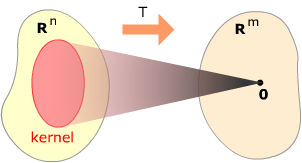
\includegraphics[width=0.5\textwidth]{img/kernel.png}
    \caption{Kernel Diagram}
\end{figure}

\defn{}{
    Let $T: V \to W$ be a linear transformation. The \textbf{range} of $T$, denoted by $\text{range}(T)$, is the set of all vectors in $W$ that are mapped to by $T$. 
    \[
        \text{range}(T) = \{T(\vec{v}) \in W : \vec{v} \in V\}
    \]
}
Note: If $T(\vec{v}) = A\vec{v}$, then $\text{range}(T) = \text{col}(A)$

\rmkb{
    Domain is the set of all possible inputs, codomain is the set of all possible outputs, and range is the set of all actual outputs.
}

\ex{
    $D^2 + D = 3I : C^{\infty} (\mathbb{R}) \to C^{\infty} (\mathbb{R})$ \\
    Find the kernel and range of $D^2 + D$.
    \[
        \ker(D^2 + D) = \{y \in C^{\infty} (\mathbb{R}) : (D^2 + D)(y) = 0\}
    \]
    \[
        = \{y \in C^{\infty} (\mathbb{R}) : y'' + y' = 0\}
    \]
}
Therefore, a homogenous linear differential equation is an example of a kernel.

\ex{
    Let $T:P_2 \to P_1$ be defined as follow:
    \[
        T(ax^2 + bx + c) = (a+b) + (b - c)x
    \] 
    Find the kernel and range of $T$. \\
    \textbf{Kernel:  } \\
    We want $(a+b) + (b - c)x = 0$ in $P_2$ \\
    Which is $0 + 0x$ in $P_1$ \\
    Therefore, $(a+b)$ and $(b-c)$ must be 0. \\
    \[
        \begin{bmatrix}
            \begin{array}{ccc|c}
                1 & 1 & 0 & 0 \\
                0 & 1 & -1 & 0
            \end{array}
        \end{bmatrix}
        =
        \begin{bmatrix}
            \begin{array}{ccc|c}
                1 & 0 & 1 & 0 \\
                0 & 1 & -1 & 0
            \end{array}
        \end{bmatrix}
    \]
    \[
        a = -c, b = c, c = c
    \]
    \[
        \ker(T) = \{-cx^2 + cx + c | c \in \mathbb{R}\}
    \]
    Write it as a spanned set: 
    \[
        \ker(T) = \text{span}\{-x^2 + x + 1\}
    \]
    \textbf{Range:}\\
    We want $(a+b) + (b - c)x$ in $P_1$ \\
    Let $b + ex $ be a generic element in $P_1$ \\
    Therefore, $d = a + b$ and $e = b - c$ \\
    We want to solve for $a, b, c$ in terms of $d, e$ \\
    \[
        \begin{bmatrix}
            \begin{array}{ccc|c}
                1 & 1 & 0 & d \\
                0 & 1 & -1 & e
            \end{array}
        \end{bmatrix}
        =
        \begin{bmatrix}
            \begin{array}{ccc|c}
                1 & 0 & 1 & d - e\\
                0 & 1 & -1 & e
            \end{array}
        \end{bmatrix}
    \]\\
    \[
        a = d - e -c, b = e + c, c \text{ is free}
    \]
    \[
        (a + b) + (b - c)x = (d - e + e + c) + (e + c - c)x = d + ex
    \]
    \[
        \text{range}(T) = \{d + ex | d, e \in \mathbb{R}\}
    \]
    So the range is all of $P_1(\mathbb{R})$.
}

\thmr{}{}{
    Let $T: V \to W$ be a linear transformation. Then:
    \begin{enumerate}
        \item $\ker(T)$ is a subspace of $V$
        \item $\text{range}(T)$ is a subspace of $W$
    \end{enumerate}
}

\pf{
    Let $T: V \to W$ be a linear transformation. \\
    1. $\ker(T)$ is a subspace of $V$ \\
    \begin{enumerate}
        \item $\vec{0_V} \in \ker(T)$ since $T(\vec{0_V}) = \vec{0_W}$
        \item Let $\vec{v}_1, \vec{v}_2 \in \ker(T)$ and $\lambda \in \mathbb{R}$. \\
        Then $T(\vec{v}_1 + \vec{v}_2) = T(\vec{v}_1) + T(\vec{v}_2) = \vec{0_W} + \vec{0_W} = \vec{0_W}$ \\
        Therefore, $\vec{v}_1 + \vec{v}_2 \in \ker(T)$ 
        \item Also, $T(\lambda\vec{v}_1) = \lambda T(\vec{v}_1) = \lambda \vec{0_W} = \vec{0_W}$ \\
        Therefore, $\lambda\vec{v}_1 \in \ker(T)$ \\
        Thus, $\ker(T)$ is a subspace of $V$.
    \end{enumerate}
    2. $\text{range}(T)$ is a subspace of $W$ 
    \begin{enumerate}
        \item $\vec{0_W} \in \text{range}(T)$ since $T(\vec{0_V}) = \vec{0_W}$
        \item Let $\vec{w}_1, \vec{w}_2 \in \text{range}(T)$ and $\lambda \in \mathbb{R}$. \\
        Then there exists $\vec{v}_1, \vec{v}_2 \in V$ such that $T(\vec{v}_1) = \vec{w}_1$ and $T(\vec{v}_2) = \vec{w}_2$. \\
        Then $T(\vec{v}_1 + \vec{v}_2) = T(\vec{v}_1) + T(\vec{v}_2) = \vec{w}_1 + \vec{w}_2$ \\
        Therefore, $\vec{w}_1 + \vec{w}_2 \in \text{range}(T)$ 
        \item Also, $T(\lambda\vec{v}_1) = \lambda T(\vec{v}_1) = \lambda \vec{w}_1$ \\
        Therefore, $\lambda\vec{w}_1 \in \text{range}(T)$ \\
        Thus, $\text{range}(T)$ is a subspace of $W$.
    \end{enumerate}

}

\ex{
    Find the basis for the range and kernel of: $D^2: P_3 \to P_3 $ given by  $D^2(p) = p''$ \\
}
\pf{
    \[
        p(x) = ax^3 + bx^2 + cx + d.
    \]
    \textbf{Basis for the Kernel:} \\
    The kernel of a linear transformation consists of all elements that map to the zero element of the codomain. For the transformation \(D^2\), we need to find all \(p \in P_3\) such that \(D^2(p) = 0\). 
    Applying \(D^2\) to the general polynomial:
    \[
    p''(x) = (ax^3 + bx^2 + cx + d)'' = (3ax^2 + 2bx + c)'' = 6ax + 2b.
    \]
    Setting \(p''(x) = 0\) yields:
    \[
    6ax + 2b = 0.
    \]
    For this to be true for all \(x\), we must have \(a = 0\) and \(b = 0\). Therefore, \(p(x)\) reduces to:
    \[
    p(x) = cx + d.
    \]

    Polynomials of the form \(cx + d\) clearly form the kernel of \(D^2\), and are elements of \(P_1\) (the space of all polynomials of degree at most 1). Hence, a basis for the kernel of \(D^2\) consists of the polynomials:
    \[
    \boxed{\{1, x\}}
    \] 
}

\pf{
    \textbf{Basis for the Range:} \\
    The range of \(D^2\) consists of all possible outputs \(D^2(p)\) for \(p \in P_3\). From the calculation above, we found:
    \[
    D^2(p) = 6ax + 2b.
    \]

    This expression tells us that the output of \(D^2\) can be any polynomial of the form \(6ax + 2b\), which can be rewritten as a linear combination of the basis \(\{x, 1\}\) (or equivalently, \(\{6x, 2\}\)).
    \[
    \boxed{\{6x, 2\}}
    \]
}

\thmr{Genearl Rank-Nullity Theorem}{Genearl Rank-Nullity Theorem}{
    Let $T: V \to W$ be a linear transformation. Then:
    \[
        \dim(V) = \dim(\ker(T)) + \dim(\text{range}(T))
    \]
}

\ex{
    Let $S : M_2(\mathbb{R}) \to M_2(\mathbb{R})$ be the transformation with the rule $S(A) = A A^T$. Find a basis for its kernel and the dimension of its range. Confirm the general rank/nullity theorem based on what we found about its kernel and range previously.

    % TODO: figure out how to prove this

    \begin{proof}
        \textbf{Kernel:} \\
        We want to find $A$ such that $AA^T = \vec{0}$. \\
        \[
            \begin{bmatrix}
                a & b \\
                c & d
            \end{bmatrix}
            \begin{bmatrix}
                a & c \\
                b & d
            \end{bmatrix}
            =
            \begin{bmatrix}
                a^2 + b^2 & ac + bd \\
                ac + bd & c^2 + d^2
            \end{bmatrix}
            =
            \begin{bmatrix}
                0 & 0 \\
                0 & 0
            \end{bmatrix}
        \]
        \[
            a^2 + b^2 = 0, ac + bd = 0, c^2 + d^2 = 0
        \]
        \[
            a = b = c = d = 0
        \]
        Therefore, the kernel is $\{0\}$ and the dimension is 0. \\
        \textbf{Range:} \\
        We want to find $A$ such that $AA^T = B$ for some $B \in M_2(\mathbb{R})$. \\
        \[
            \begin{bmatrix}
                a & b \\
                c & d
            \end{bmatrix}
            \begin{bmatrix}
                a & c \\
                b & d
            \end{bmatrix}
            =
            \begin{bmatrix}
                a^2 + b^2 & ac + bd \\
                ac + bd & c^2 + d^2
            \end{bmatrix}
        \]
        The basis for it will be: \\
        \[
            \begin{Bmatrix}
                \begin{bmatrix}
                    1 & 0 \\
                    0 & 0
                \end{bmatrix}
                \begin{bmatrix}
                    0 & 1 \\
                    1 & 0
                \end{bmatrix}
                \begin{bmatrix}
                    0 & 0 \\
                    0 & 1
                \end{bmatrix}
            \end{Bmatrix}
        \]
        Therefore, the range is all of $M_2(\mathbb{R})$ and the dimension is 4. \\
        \textbf{Rank-Nullity Theorem:} \\
        \[
            \dim(M_2(\mathbb{R})) = \dim(\ker(S)) + \dim(\text{range}(S))
        \]
        \[
            \boxed{4 \neq 0 + 3}
        \]
        
    \end{proof}

    This is not a linear transformation because it does not satisfy the properties of linearity. Therefore, the rank-nullity theorem does not hold.


}


\ex{
    Consider the linear transformation $T : M_2(\mathbb{R}) \to P_2(\mathbb{R})$ given by \\ 
    \[
        T\begin{pmatrix}
            \begin{bmatrix} a & b \\ c & d \end{bmatrix}
        \end{pmatrix} = (a - b + d) + ( - a + b - d)x^2
    \]
    Determine $\text{range}(T)$. What is the dimension of $\ker(T)$? Determine a basis for $\ker(T)$.

    % \begin{proof}
    %     \textbf{Kernel:} \\
    %     We want to find $A$ such that $T(A) = 0$. \\
    %     \[
    %         (a - b + d) + ( - a + b - d)x^2 = 0
    %     \]
    %     \[
    %         a - b + d = 0, -a + b - d = 0
    %     \]
    %     \[
    %         a = b = d = 0
    %     \]
    %     Therefore, the kernel is $\begin{bmatrix} 0 & 0 \\ 1 & 0 \end{bmatrix}$ and the dimension is 1. \\
    %     \textbf{Range:} \\
    %     We want to find $A$ such that $T(A) = p(x)$. \\
    %     \[
    %         (a - b + d) + ( - a + b - d)x^2 = p(x)
    %     \]
    %     Let $y = a - b + d$ and $z = -a + b - d$. \\
    %     Therefore, the range is all of $P_2(\mathbb{R})$ and the dimension is 2. \\
    %     \textbf{Rank-Nullity Theorem:} \\
    %     \[
    %         \dim(M_2(\mathbb{R})) = \dim(\ker(T)) + \dim(\text{range}(T))
    %     \]
    % \end{proof}

    Step 1: Verify it is linear: \\
    Let $A = \begin{bmatrix} a_1 & b_1 \\ c_1 & d_1 \end{bmatrix}$ and $B = \begin{bmatrix} a_2 & b_2 \\ c_2 & d_2 \end{bmatrix}$ \\
    \[
        T(A + B) = T\begin{pmatrix}
            \begin{bmatrix} a_1 + a_2 & b_1 + b_2 \\ c_1 + c_2 & d_1 + d_2 \end{bmatrix}
        \end{pmatrix}
        = (a_1 + a_2 - b_1 - b_2 + d_1 + d_2) + (-a_1 - a_2 + b_1 + b_2 - d_1 - d_2)x^2
    \]
    \[
        T(A) + T(B) = T\begin{pmatrix}
            \begin{bmatrix} a_1 & b_1 \\ c_1 & d_1 \end{bmatrix}
        \end{pmatrix} + T\begin{pmatrix}
            \begin{bmatrix} a_2 & b_2 \\ c_2 & d_2 \end{bmatrix}
        \end{pmatrix}
        = (a_1 - b_1 + d_1) + (-a_1 + b_1 - d_1)x^2 + (a_2 - b_2 + d_2) + (-a_2 + b_2 - d_2)x^2
    \]
    \[
        (a_1 + a_2 - b_1 - b_2 + d_1 + d_2) + (-a_1 - a_2 + b_1 + b_2 - d_1 - d_2)x^2
    \]
    \[
        T(A + B) = T(A) + T(B)
    \]
    Therefore, $T$ is linear. \\

}



\subsection{Linear transformation and basis}

If we have a matrix $A$ that's $m$ by $n$, we get a free transformation. 
$T: f_n \to f_m$ given by $T(x) = Ax$ if $V$ and $W$ are finite-dimensional, then $T: V \to W$ can be accomplished by a matrix multiplication. That is there exist a matrix $A$ such that $T(\vec{v}) = A\vec{v}$ for all $\vec{v} \in V$.

% We have seen that, given an m × n matrix A, we can define a linear transformation T : Rn → Rm by T (v) = Av. (Remember that an m × n matrix maps R n
% to R
% m
% .)
% Now, given a linear transformation T : Rn → Rm, we identify an m × n matrix A such that T (v) = Av.
% This is possible, because if we know how T acts on a basis {b1, . . . , bn} of V , then we know how T acts on the whole of V , since if v = c1b1 + . . . ckbk, then
% T (v) = T (c1b1 + . . . ckbk) = c1T (b1) + . . . ckT (bk).
% In particular, if T : Rn → Rm and if v = (c1, c2, . . . , cn) = c1e1 + c2e2 + · · · + cnen, then
% T (v) = T (c1e1 + c2e2 + · · · + cnen) = c1T (e1) + c2T (e2) + · · · + cnT (en) .
% By the definition of matrix multiplication, the boxed expression is equal to
%   c1   [T (e1)|T (e2)| · · · |T (en)]
%  c2   .   . .
% .
% 
% cn
% Then T (v) = Av where A = [T (e1)|T (e2)| · · · |T (en)]. 

\thmr{}{}{
    Let $T : \mathbb{R}^n \to \mathbb{R}^m$ be a linear transformation. Then there exists an $m \times n$ matrix $A$ such that $T(v) = Av$ for all $v \in \mathbb{R}^n$.
}


We have seen that, given an $m \times n$ matrix A, we can define a linear transformation $T : \mathbb{R}^n \to \mathbb{R}^m$ by $T(v) = Av$. (Remember that an $m \times n$ matrix maps $\mathbb{R}^n$ to $\mathbb{R}^m$.) 

Now, given a linear transformation $T : \mathbb{R}^n \to \mathbb{R}^m$, we identify an $m \times n$ matrix A such that $T(v) = Av$. 

This is possible, because if we know how T acts on a basis $\{b_1, \cdots, b_n\}$ of $V$, then we know how T acts on the whole of $V$, since if $v = c_1b_1 + \cdots + c_kb_k$, then 

\[
    T(v) = T(c_1b_1 + \cdots + c_kb_k) = c_1T(b_1) + \cdots + c_kT(b_k)
\]

In particular, if $T : \mathbb{R}^n \to \mathbb{R}^m$ and if $v = (c_1, c_2, \cdots, c_n) = c_1e_1 + c_2e_2 + \cdots + c_ne_n$, then

\[T(v) = T(c_1e_1 + c_2e_2 + \cdots + c_ne_n) = \boxed{c_1T(e_1) + c_2T(e_2) + \cdots + c_nT(e_n)}\]

By the definition of matrix multiplication, the boxed expression is equal to

\[
    \begin{bmatrix}
        T(e_1) & T(e_2) & \cdots & T(e_n)
    \end{bmatrix}
    \begin{bmatrix}
        c_1\\
        c_2\\
        \vdots\\
        c_n
    \end{bmatrix}
\]

Then $T(v) = Av$ where $A = \begin{bmatrix} T(e_1) & T(e_2) & \cdots & T(e_n) \end{bmatrix}$.








\ex{
    Find $A$. $T_1 \mathbb{R}^2 \to \mathbb{R}^2$ \\
    \[
        T(x) = \beta 
    \]
    \[
        \beta = \{\vec{e_1}, \vec{e_2}, \cdots , \vec{e_n}\}
    \]
    \[
        T(x) = (a_1 \cdot e_1 + a_2 \cdot e_2 + \cdots + a_n \cdot e_n)
    \]
    \[
        = a_1 T(\vec{e_1}) + a_2 T(\vec{e_2}) + \cdots + a_n T(\vec{e_n})
    \]
    \[
        A = \begin{bmatrix}
            T(\vec{e_1}) & T(\vec{e_2}) & \cdots & T(\vec{e_n})
        \end{bmatrix}
    \]
    If I take the matrix A and apply it to the coefficient vector, I get the transformation.
    \[
        A \cdot
        \begin{bmatrix}
            a_1\\
            a_2\\
            \vdots\\
            a_n
        \end{bmatrix}
        = 
        \begin{bmatrix}
            T(\vec{e_1}) & T(\vec{e_2}) & \cdots & T(\vec{e_n})
        \end{bmatrix}
        \begin{bmatrix}
            a_1\\
            a_2\\
            \vdots\\
            a_n
        \end{bmatrix}
    \]
    \[
        = a_1 T(\vec{e_1}) + a_2 T(\vec{e_2}) + \cdots + a_n T(\vec{e_n})
    \]
    \[
        = T(a_1 \vec{e_1} + a_2 \vec{e_2} + \cdots + a_n \vec{e_n})
    \]

}


% Find a matrix A such that T (x) = A(x) where T : R3 → R2, is given by T (a, b, c) = (c, a + b).

\ex{
    Find a matrix $A$ such that $T(x) = A(x)$ where $T : \mathbb{R}^3 \to \mathbb{R}^2$ is given by $T(a, b, c) = (c, a + b)$.\\

    Since this is from $\mathbb{R}^3$ to $\mathbb{R}^2$, the matrix $A$ will be $2 \times 3$. \\
    \[
        T(a, b, c) = (c, a + b)
    \]
    \[
        A = \begin{bmatrix}
            T(\vec{e_1}) & T(\vec{e_2}) & T(\vec{e_3})
        \end{bmatrix}
    \]
    \[
        A = \begin{bmatrix}
            T(1, 0, 0) & T(0, 1, 0) & T(0, 0, 1)
        \end{bmatrix}
    \]
    \[
        =A = \begin{bmatrix}
            0 & 1 & 0\\
            1 & 1 & 0
        \end{bmatrix}
    \]
    \[
        A \cdot \begin{bmatrix}
            a\\
            b\\
            c
        \end{bmatrix}
        = \begin{bmatrix}
            0 & 1 & 0\\
            1 & 1 & 0
        \end{bmatrix}
        \begin{bmatrix}
            a\\
            b\\
            c
        \end{bmatrix}
    \]
    \[
        \begin{bmatrix}
            c\\
            a + b
        \end{bmatrix}
    \]
    \[
        \boxed{= (c, a + b)}
    \]
    

    
}
\newpage